\documentclass[20pt,a1paper,portrait,margin=2mm, innermargin=18mm,
blockverticalspace=15mm, colspace=15mm, subcolspace=8mm]{tikzposter} % See Section 3

\usepackage[utf8]{inputenc}
%\usepackage{cite}
\usepackage{pifont}
\usepackage{xcolor}
\usepackage{graphicx}
\usepackage{tikz}
\usetikzlibrary{arrows,automata,positioning,calc,shapes,snakes}

\usepackage{amssymb,amsthm,amsmath}


%%%%%%%%%%%%%%%%%%%%%%%%%%%%%%%%%%%%%%%%%%%%%%%

\title{\parbox{0.9\linewidth}{\centering The economic Style of my\\ very first Poster}}
\institute{Artificial Intelligence Group, University of Hagen} 
\author{Lydia Bl\"umel}


%%%%%%%%%%%%%%%%%%%%%%%%%%%%%%%%%%%%%%%%%%%%%%%%%%%%%%%%%%%%%%



%Titlemaking
\definetitlestyle{aighagen}{roundedcorners=0, linewidth=5pt, innersep=5pt,
	titletotopverticalspace=0mm, titletoblockverticalspace=30mm
}{
\begin{scope}[line width=\titlelinewidth, rounded corners=\titleroundedcorners]
	\draw[color=blocktitlebgcolor, fill=titlebgcolor]
	(\titleposleft,\titleposbottom) rectangle (\titleposright,\titlepostop);
\end{scope}
}

\makeatletter
\renewcommand\TP@maketitle{%
	\begin{minipage}{0.7\linewidth}
		\centering
		\color{titlefgcolor}
		\vspace*{0.7em}
		{\bfseries \Huge \sc \@title \par}
		\vspace*{1.5em}
		{\huge \@author \par}
		\vspace*{0.8em}
		{\LARGE \@institute}
	\end{minipage}%
	\hfill
	\begin{minipage}{0.3\linewidth}
		\centering
		
\includegraphics[scale=0.9]{figures/logoaig.png}
	\end{minipage}
}
\makeatother

\usetitlestyle{aighagen}


%Blocks


%Colors
\definecolorstyle{aigposter} {
	\definecolor{aigyellow}{RGB}{210,149,81}
	\definecolor{aigblue}{RGB}{0,76,151}
}{
	% Background Colors
	\colorlet{backgroundcolor}{white}%{aigblue!30!white}
	\colorlet{framecolor}{aigblue}
	% Title Colors
	\colorlet{titlefgcolor}{aigblue}
	\colorlet{titlebgcolor}{white}
	% Block Colors
	\colorlet{blocktitlebgcolor}{aigblue}
	\colorlet{blocktitlefgcolor}{white}
	\colorlet{blockbodybgcolor}{aigblue!30!white}
	\colorlet{blockbodyfgcolor}{black}
	% Innerblock Colors
	\colorlet{innerblocktitlebgcolor}{white}
	\colorlet{innerblocktitlefgcolor}{aigblue}
	\colorlet{innerblockbodybgcolor}{white}
	\colorlet{innerblockbodyfgcolor}{black}
}
\usecolorstyle{aigposter}
\usebackgroundstyle{VerticalGradation}
%\usetheme{Basic} 



\begin{document}
	
\maketitle % See Section 4.1
	
	
	
%	\block{Abstract}{Blocktext} % See Section 4.2
	
	\begin{columns}
	\column{0.35}
	
	\block{Example Block A}{
	
		
		\begin{tikzfigure}[A tikz-picture of an AF]
			\label{Fig1:Figure 1}
			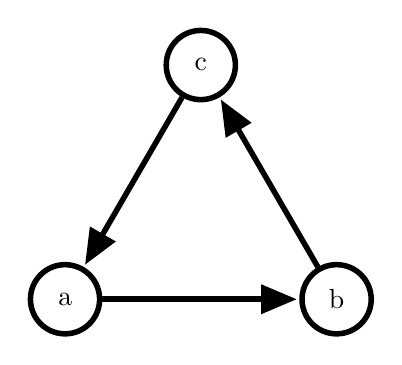
\begin{tikzpicture}[->,>=triangle 45,shorten >=1pt,auto,
				thick]
				\pgfsetlinewidth{2pt}
				\tikzstyle{every state}=[fill=white,draw=black,text=black]
				\node[state]   (A) {a};
				\node[state]   (B) [right = 2.5cm of A]  {b};
				\node[state]   (C) [above = 2.5cm of {$(A)!0.5!(B)$}] {c};
				
				\path (A) edge node {} (B)
				(C) edge node {} (A)
				(B) edge node {} (C);
			\end{tikzpicture}
		\end{tikzfigure}
}
	
	\column{0.65}
	
	\block{Example Block B}{
		Normal text.\vspace{5pt}
		
		
		\begin{itemize}
			\item an item
		\end{itemize}
	    
	    \begin{description}
	    	\item[item] description
	    \end{description}
    
        \begin{enumerate}
        	\item an enumerated item
        \end{enumerate}
	}
	\end{columns}
	
	\begin{columns} % See Section 4.4
		\column{0.6} % See Section 4.4
		

		\block{Example Block C}{ 
			An equation
			\begin{equation} 
			     \Delta{esign}\quad \Longleftrightarrow\quad \bigcup_{ti}{lity}\ \cup\ Aesthetics  
			\end{equation} 	
		
		
		A table\vspace{5pt}
	   \begin{center}	
		\begingroup
		\renewcommand{\arraystretch}{1.7}
		
		\begin{tabular}{c|c}
			 \textbf{Column 1}  & \textbf{Column 2}	\\ \hline
			 Entry 1 & Entry 2
		\end{tabular}
	\endgroup
	\end{center}
	\vspace{5pt}
	   
       A table as an inner block\\
       
       \innerblock{\centering
       	\begin{tabular}{c | c}
       		\textbf{Column 1}  & \textbf{Column 2}	\\ \hline
       		Entry 1 & Entry 2 \\
       	\end{tabular}
       } 
   } 

	
 



		
\column{0.4}
		
		


\block{Block D}{
	For discussing "fancy" stuff formats like
\begin{itemize}	
	\item[\ding{228}] cooler itemize versions
\end{itemize}
}

\block{TODO}{
	
	\begin{itemize}	
		\item create a .sty-file
		\item decide on a blockstyle
		\item add highlight-colors
		\item check compatibility with a0-format
		\item add working referencing solution
		\item add examples for manipulating positioning 
	\end{itemize}
}

%Contact block, may want to include references or a QR-Code for building or?
\block[roundedcorners=0]{}{
\textbf{Contact me} lydia.bluemel@fernuni-hagen.de\\
   or via Teams
}

\end{columns}

\end{document}